% \section{Dataset Reservoir and Standardization}

% \subsection{Ground-truth filtering}

% \arena{} begins from a large candidate pool and filters tasks according to ground-truth availability and evaluation readiness. A task is retained if it has a valid ground-truth formula, train/ID/OOD splits, usable metadata, and a parsable expression representation. This yields
% \[
% D_{\mathrm{GT}} = 664.
% \]
% The resulting \reservoir{} is the population that \core{} is designed to represent.

% Reservoir composition is audited by source family, operator profile, formula complexity, and probe-derived difficulty bins. We keep the detailed composition plot in \cref{app:additional-figures} so the main text can focus on the distillation and validation evidence.

% \subsection{Metadata and expression standardization}

% Each dataset stores at least the following fields:
% \begin{verbatim}
% dataset_id, family, subgroup, basename, source_benchmark,
% ground_truth_formula, train_split, id_test_split, ood_test_split,
% n_features, sample_count, formula_complexity, operator_types,
% ood_type, dummy_variable_flag, semantic_duplicate_group
% \end{verbatim}

% All formulas are canonicalized into a unified expression representation, including canonical strings, prefix/postfix forms, expression trees, operator-normalized forms, constant-normalized forms, and Newick-like tree formats. This standardization enables symbolic equivalence testing, expression-tree comparison, operator and variable recovery, duplicate detection, and seed-level structural consistency.
\section{Dataset Reservoir and Standardization}
\label{sec:reservoir}

\arena{} begins from a large candidate pool of more than 800 symbolic regression tasks and filters them by ground-truth availability and evaluation readiness. A task is retained if it provides a valid ground-truth formula, fixed train/ID/OOD splits, usable metadata, and a parsable expression representation. This yields $|D_{\mathrm{GT}}| = 664.$

The resulting \reservoir{} is the parent population that \core{} is designed to represent. Its composition is audited by source family, operator profile, formula complexity, and difficulty bins; detailed statistics are provided in \cref{app:reservoir}.

Each retained dataset stores standardized provenance, split, formula, and structural metadata. All formulas are canonicalized into a unified expression representation, including canonical strings, prefix/postfix forms, expression trees, operator-normalized forms, constant-normalized forms, and Newick-like tree serializations. This standardization enables symbolic equivalence testing, expression-tree comparison, operator and variable recovery, duplicate detection, and seed-level structural consistency in later leaderboard evaluation. Detailed reservoir composition statistics are provided in \cref{fig:appendix-reservoir-composition}.

\begin{figure}[t]
\centering
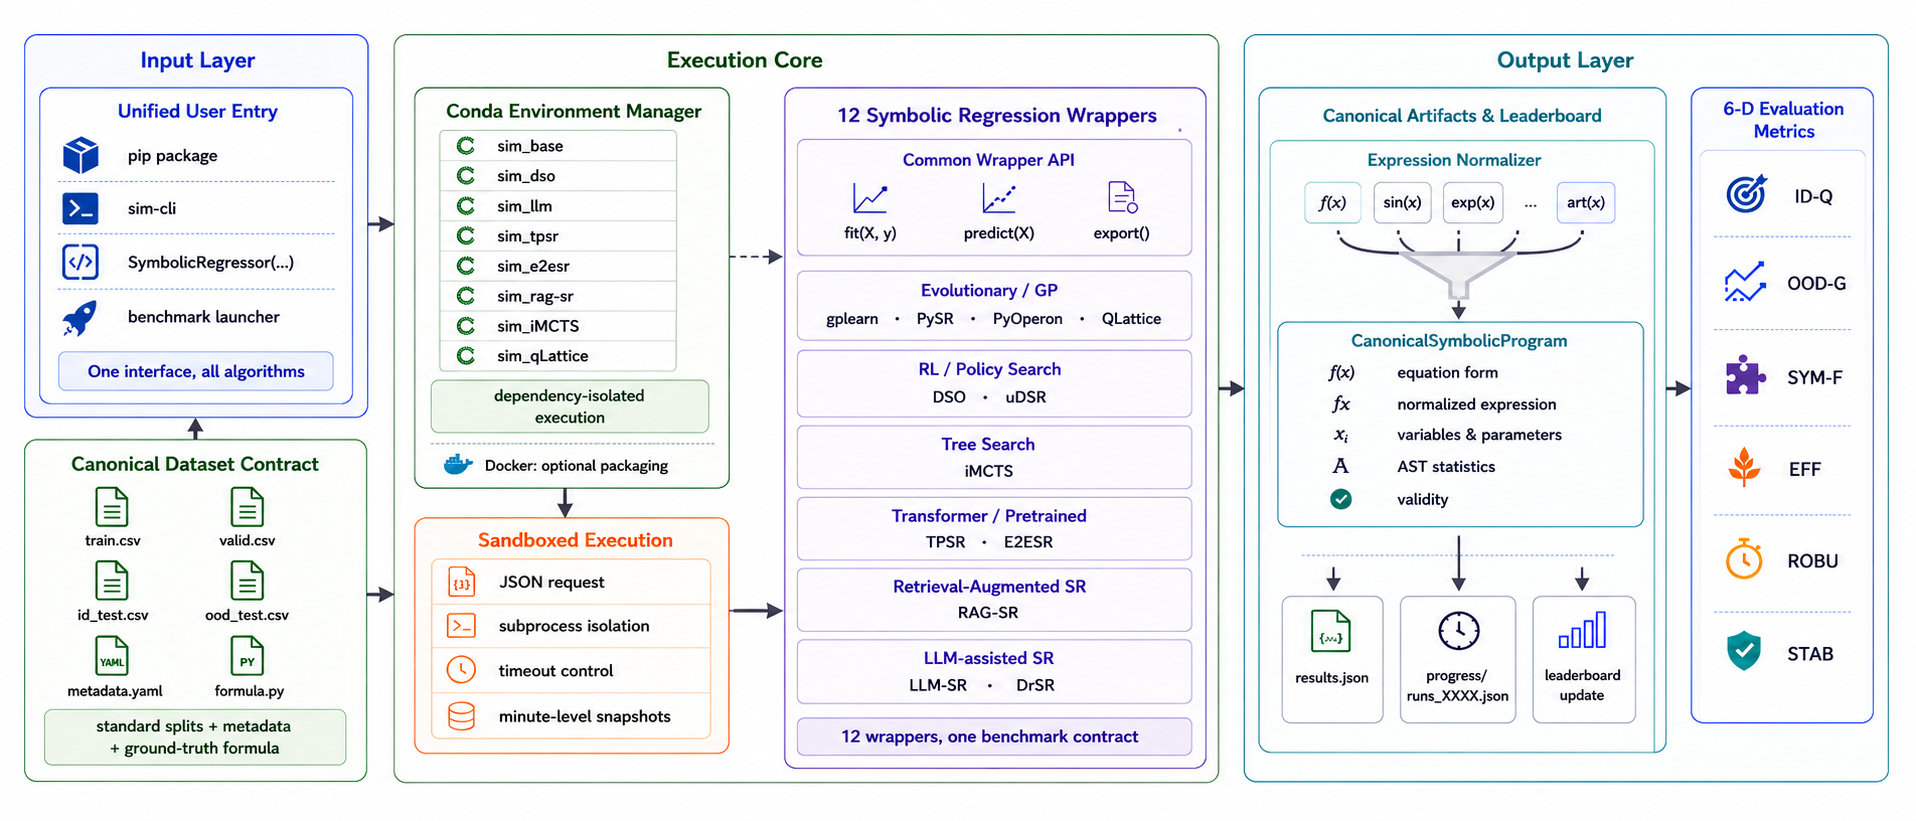
\includegraphics[width=0.95\linewidth]{imgs/Article/SAinfrastructure}
\caption{\textbf{\arena{} dataset reservoir and standardization pipeline.} Raw SR task sources are converted into a shared executable schema with validated splits, ground-truth formulas, metadata, canonical expression artifacts, and duplicate-control identities before entering benchmark distillation and leaderboard evaluation.}
\label{fig:sa-infrastructure}
\end{figure}
